\documentclass[11pt,a4paper]{article}
\usepackage[utf8]{inputenc}
\usepackage[spanish,es-sloppy]{babel}
\usepackage{amsmath}
\usepackage{amsfonts}
\usepackage{amssymb}
\usepackage{graphicx}
\usepackage{tcolorbox}
\usepackage{here}
\usepackage{tikz}
\usepackage{url}
\usepackage{pgfplots}
\usepackage{cite}
\usepackage[left=1.8cm,right=1.8cm,top=1.5cm,bottom=1.5cm]{geometry}
\usepackage{verbments}

\newcommand{\mrm}{\mathrm}
%\definecolor{fondo1}{rgb}{0.9764, 0.9764, 0.9762}
%\definecolor{fondo2}{rgb}{0.1647, 0.4980, 0.7}
\definecolor{fondo1}{rgb}{0.88, 0.88, 0.88}
\definecolor{fondo2}{rgb}{0.15, 0.15, 0.5}
\author{Josue Huaroto Villavicencio - 20174070I\\Sección: E}
\title{5$^{\circ}$ Práctica de Cálculo por Elementos Finitos - MC516}
\begin{document}
\fvset{frame=bottomline, framerule=0.02cm,numbers=left, numbersep=8pt}
\plset{language=python,texcl=true,listingnamefont=\sffamily\bfseries\color{white},captionbgcolor=fondo2, bgcolor=fondo1,listingname=\textbf{Código}, captionfont=\sffamily\color{white},fontsize=\normalsize}
\tcbset{colframe=black!50!gray,colback=gray!20,colupper=black,fonttitle=\bfseries,nobeforeafter,center title}
\maketitle
%\tableofcontents
%\section{Diagrama de flujo}
%\begin{figure}[H]
%    \centering
%    \includegraphics[scale = 1.75]{Flow.pdf}
%    \caption{Diagrama de flujo}
%\end{figure}
\section{Análisis analítico}
De las ecuaciones de equlibrio de la estática:
\begin{align*}
    R_{1} &= -R_{2}\\
    R_{2}\times 1000 &= -M\\
    R_{2} &= -200\,\mrm{N}\\
    R_{1} &= 200\,\mrm{N}
\end{align*}
Se halla los correspondientes diagramas de momento flector y de fuerza cortante.
\begin{figure}[H]
    \centering
    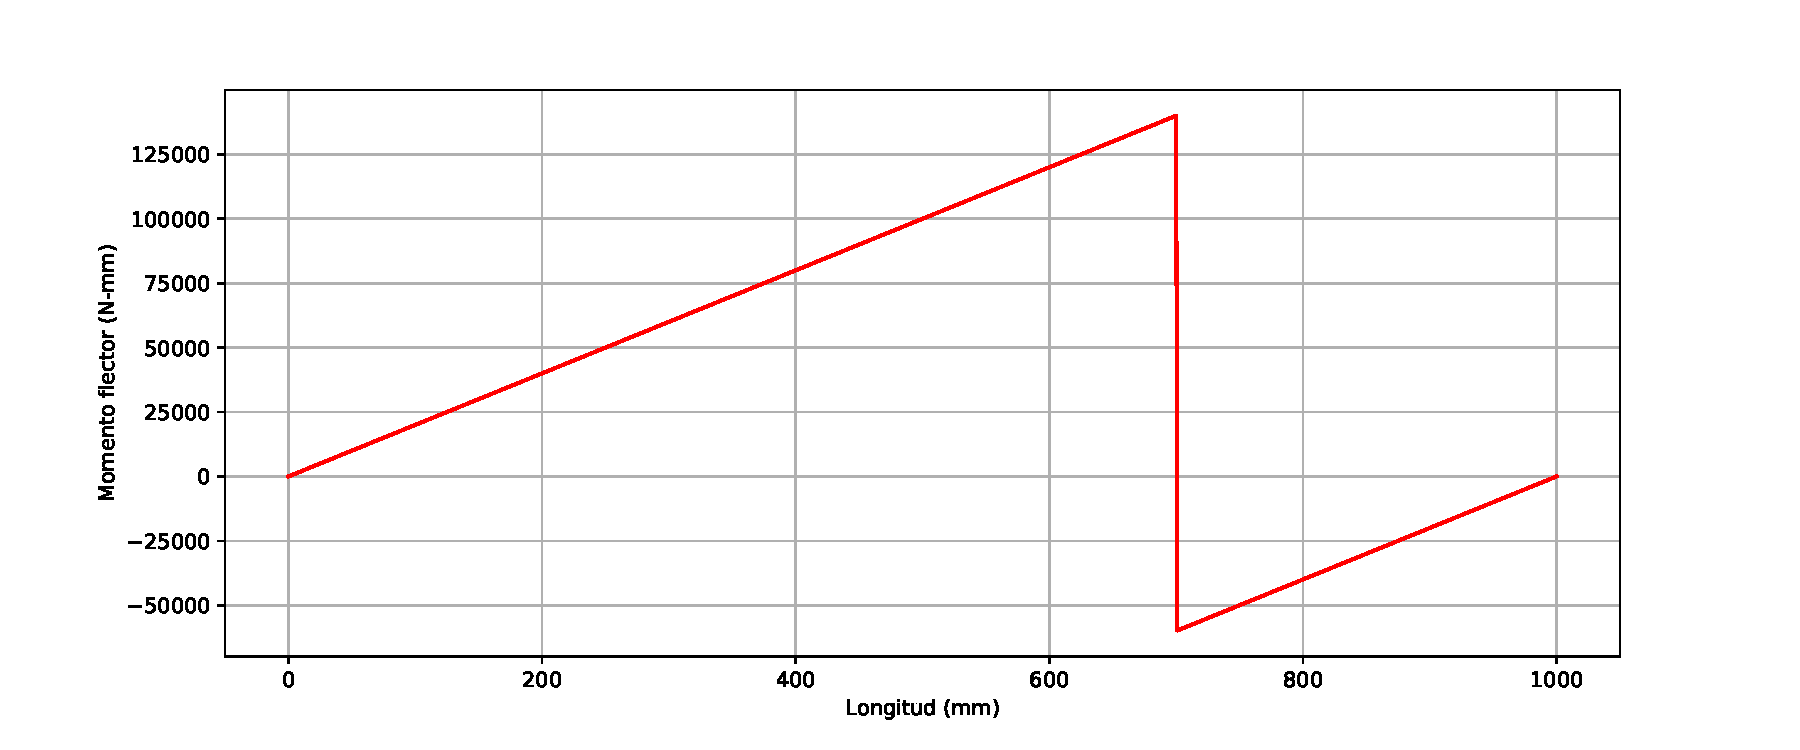
\includegraphics[scale=0.73]{dm.pdf}
    \caption{Diagrama de momento flector}
\end{figure}
\begin{figure}[H]
    \centering
    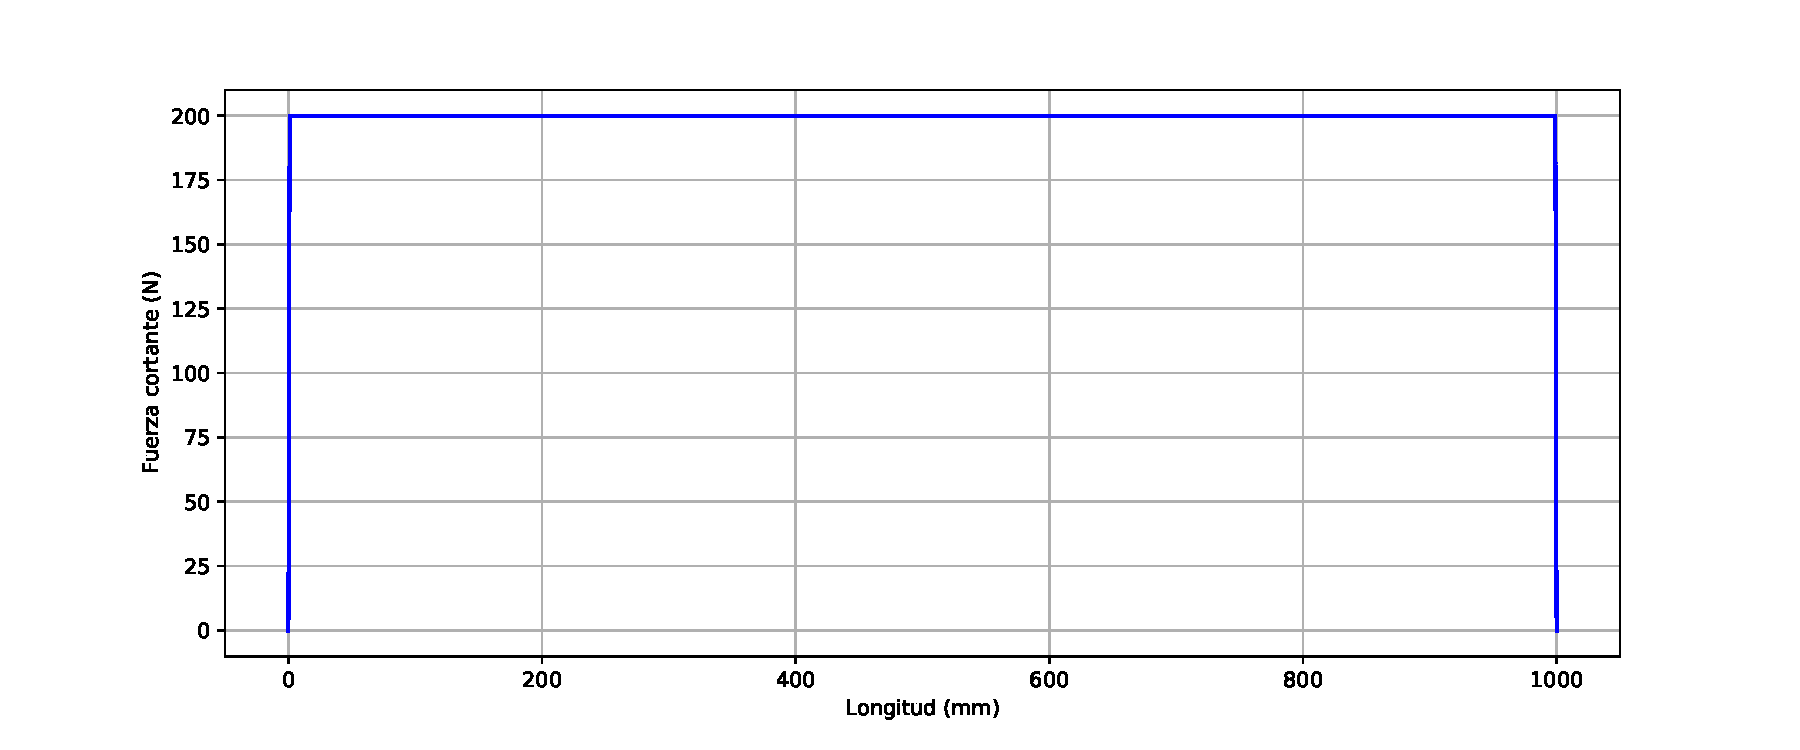
\includegraphics[scale=0.73]{dv.pdf}
    \caption{Diagrama de fuerza cortante}
\end{figure}
Luego, reescribiendo la función $M(x)$:
\begin{equation}
M(x) = R_{1}<x-0>^{1} - M <x-700>^{0} + R_{2} <x+1000>^{1}
\end{equation}
La ecuación diferencial correspondiente a la deformada de una viga:
\begin{align}
    EI\frac{\mrm{d}y^{2}}{\mrm{d}x^{2}} &= M(x)\\
    y(x) &= \frac{1}{EI}\iint M(x) \mrm{d}x \;\mrm{d}x\\
    y(x) &= \frac{\frac{R_{1}x^{3}}{6} + c_{1}x + c_{2}}{EI} \;\;\vert \;\; x \leq 700\\
    y(x) &= \frac{\frac{R_{1}x^{3}}{6} - \frac{Mx^{2}}{2} + c_{3}x + c_{4}}{EI} \;\;\vert \;\;x \geq 700
\end{align}
De las condiciones de frontera:
\begin{align}
    c_{2} &= 0\\
    c_{3} - 700M &= c_{1}\\
    c_{4} &= -49\times 10^{9}\\
    c_{3} &= 115666666.66667\\
    c_{1} &= -24333333.3333 \\
    y(x) &= \begin{cases}
    3.536068\cdot 10^{-11} x^{3} - 2.58133 \cdot 10^{-5}x & x \leq 700\\
    3.536068\cdot 10^{-11} x^{3} - 1.06082 \cdot 10^{-7} x^{2} + 1.227 \cdot 10^{-4}x - 0.0519802 & x \geq 700
    \end{cases}
\end{align}
\begin{center}
\begin{tikzpicture}
\begin{axis}[
    height=7cm,
    width=16.5cm,
    axis lines = left,
    xlabel = Posición (mm),
    ylabel = {Deformada (mm)},
]
\addplot [
    domain=0:700, 
    samples=200, 
    color=red,
    line width=1.5,
]
{3.536067892753612*10^(-11)*x^3-2.581329561710133*10^(-5)*x};
\addlegendentry{$x \leq 700$}
\addplot [
    domain=700:1000, 
    samples=200, 
    color=blue,
    line width=1.5,
]
{3.536067892753612*10^(-11)*x^3-1.0608203678260834*10^(-7)*x^2+1.2270155587855386*10^(-4)*x-0.05198019802347809};
\addlegendentry{$x \geq 700$}
\end{axis}
\end{tikzpicture}
\end{center}
Derivando la ecuación (4), se obtiene el valor de la flecha máxima y su posición en la viga:
\begin{align*}
    x_{\max} &= 493.28828623 \\
    y_{\max} &= 0.0084889329
\end{align*}
Derivando la ecuación (11), se obtiene la gráfica de la pendiente de la deformada:
\begin{equation}
    \theta (x) = \begin{cases}
    10.60820368\cdot 10^{-11} x^{2} - 2.58132956 \cdot 10^{-5} & x \leq 700\\
    10.60820368\cdot 10^{-11} x^{2} - 2.1216407\cdot 10^{-7} x + 1.227 \cdot 10^{-4} & x \geq 700
    \end{cases}
\end{equation}
Siendo la pendiente en $L_{1} = 700$mm, igual a $2.61669 \times 10^{-5}$.
\begin{center}
\begin{tikzpicture}
\begin{axis}[
    height=7cm,
    width=16.5cm,
    axis lines = left,
    xlabel = Posición (mm),
    ylabel = {Pendiente},
]
\addplot [
    domain=0:700, 
    samples=200, 
    color=red,
    line width=1.5,
]
{10.608203678260837*10^(-11)*x^2 - 2.581329561710133*10^(-5)};
\addlegendentry{$x \leq 700$}
\addplot [
    domain=700:1000, 
    samples=200, 
    color=blue,
    line width=1.5,
]
{10.608203678260837*10^(-11)*x^(2) - 2.121640735652167*10^(-7)*x + 1.2270155587855386*10^(-4)};
\addlegendentry{$x \geq 700$}
\end{axis}
\end{tikzpicture}
\end{center}
\section{Ejecución del código}
Se agrega al solver principal una nueva función llamada DFBoundaryCondition que se utilizará para agregar una fuerza distribuida sobre un elemento.
\begin{pyglist}[language=python,caption={Carga distribuida sobre un elemento},style=pastie]
def DFBoundaryCondition(nF,w,e):
    f = Elements[e][0]
    s = Elements[e][1]
    l = L[e]
    FBoundaryCondition(nF,w*l/2,2*f+0)
    FBoundaryCondition(nF,w*l*l/12,2*f+1)
    FBoundaryCondition(nF,w*l/2,2*s+0)
    FBoundaryCondition(nF,-w*l*l/12,2*s+1)
\end{pyglist}
Ahora, es necesario modificar la inserción de las matrices de rigidez de los elementos a la matriz de rigidez global.
\begin{pyglist}[language=python,caption={Ensamble de la matriz de rigidez},style=pastie]
def ElementStiffness(E, I, L):
    aux = np.zeros((4,4))
    s1 = np.array([12,6*L,-12,6*L])
    s2 = np.array([6*L,4*L*L,-6*L,2*L*L])
    for i in range(0,2):
        for j in range(0,4):
            aux[2*i][j] = s1[j]
            aux[2*i+1][j] = s2[j]
            if(i == 1):
                aux[2*i][j] *= -1
    aux[3][1] = 2*L*L
    aux[3][3] = 4*L*L
    aux = aux*E*I/(L**3)
    return aux

def AssemblyStiffness(nStiffnessMatrix,k,i,j):
    for p in range(0,2):
        for m in range(0,2):
            nStiffnessMatrix[2*i+p][2*i+m] += k[p][m]
            nStiffnessMatrix[2*i+p][2*j+m] += k[p][2+m]
            nStiffnessMatrix[2*j+p][2*i+m] += k[p+2][m]
            nStiffnessMatrix[2*j+p][2*j+m] += k[p+2][2+m]
\end{pyglist}
Todos los demás elementos del código permanecen igual; ahora solo se necesita definir las condiciones del problema a resolver.
\begin{pyglist}[language=python,caption={Condiciones del problema},style=pastie]
NodesCondition = []
Nodes = 1001
Nodes *= 2
NumberOfElement = 1000

E = 3e5 #MPA
K = []
I = 314.2222e4 #mm$^{4}$
M_A = 2e5 #N-mm
PosNodes = np.linspace(0,1000,NumberOfElement+1)
Elements = []
for i in range(0,NumberOfElement):
    Elements.append((i,i+1))
Elements = np.array(Elements)

L = []

for i in range(NumberOfElement):
    L.append(PosNodes[Elements[i][1]] - PosNodes[Elements[i][0]])

L = np.array(L)

for i in range(0,NumberOfElement):
    aux = ElementStiffness(E,I,L[i])
    K.append(aux)

StiffnessMatrix = np.zeros((Nodes,Nodes))

U = np.zeros(Nodes).reshape(Nodes,1)
F = np.zeros(Nodes).reshape(Nodes,1)

Initialize(StiffnessMatrix,U,F)


UBoundaryCondition(U,0,2*0+0) #Nodo 0 en Y
UBoundaryCondition(U,0,2*NumberOfElement+0) #Nodo 1000 en Y

FBoundaryCondition(F,M_A,int(2*NumberOfElement*700/1000)+1) #Momento en el nodo 700

U,F=Solve(StiffnessMatrix,U,F)
print("Stiffness Matrix:\n",StiffnessMatrix,'\n')
print("Displacements:\n",U,'\n')
print("Forces:\n",F)
\end{pyglist}

\section{Resultados del problema}
Al finalizar la ejecución del solver, obtenemos la matriz de rigidez, las fuerzas y desplazamientos:
\begin{figure}[H]
    \centering
    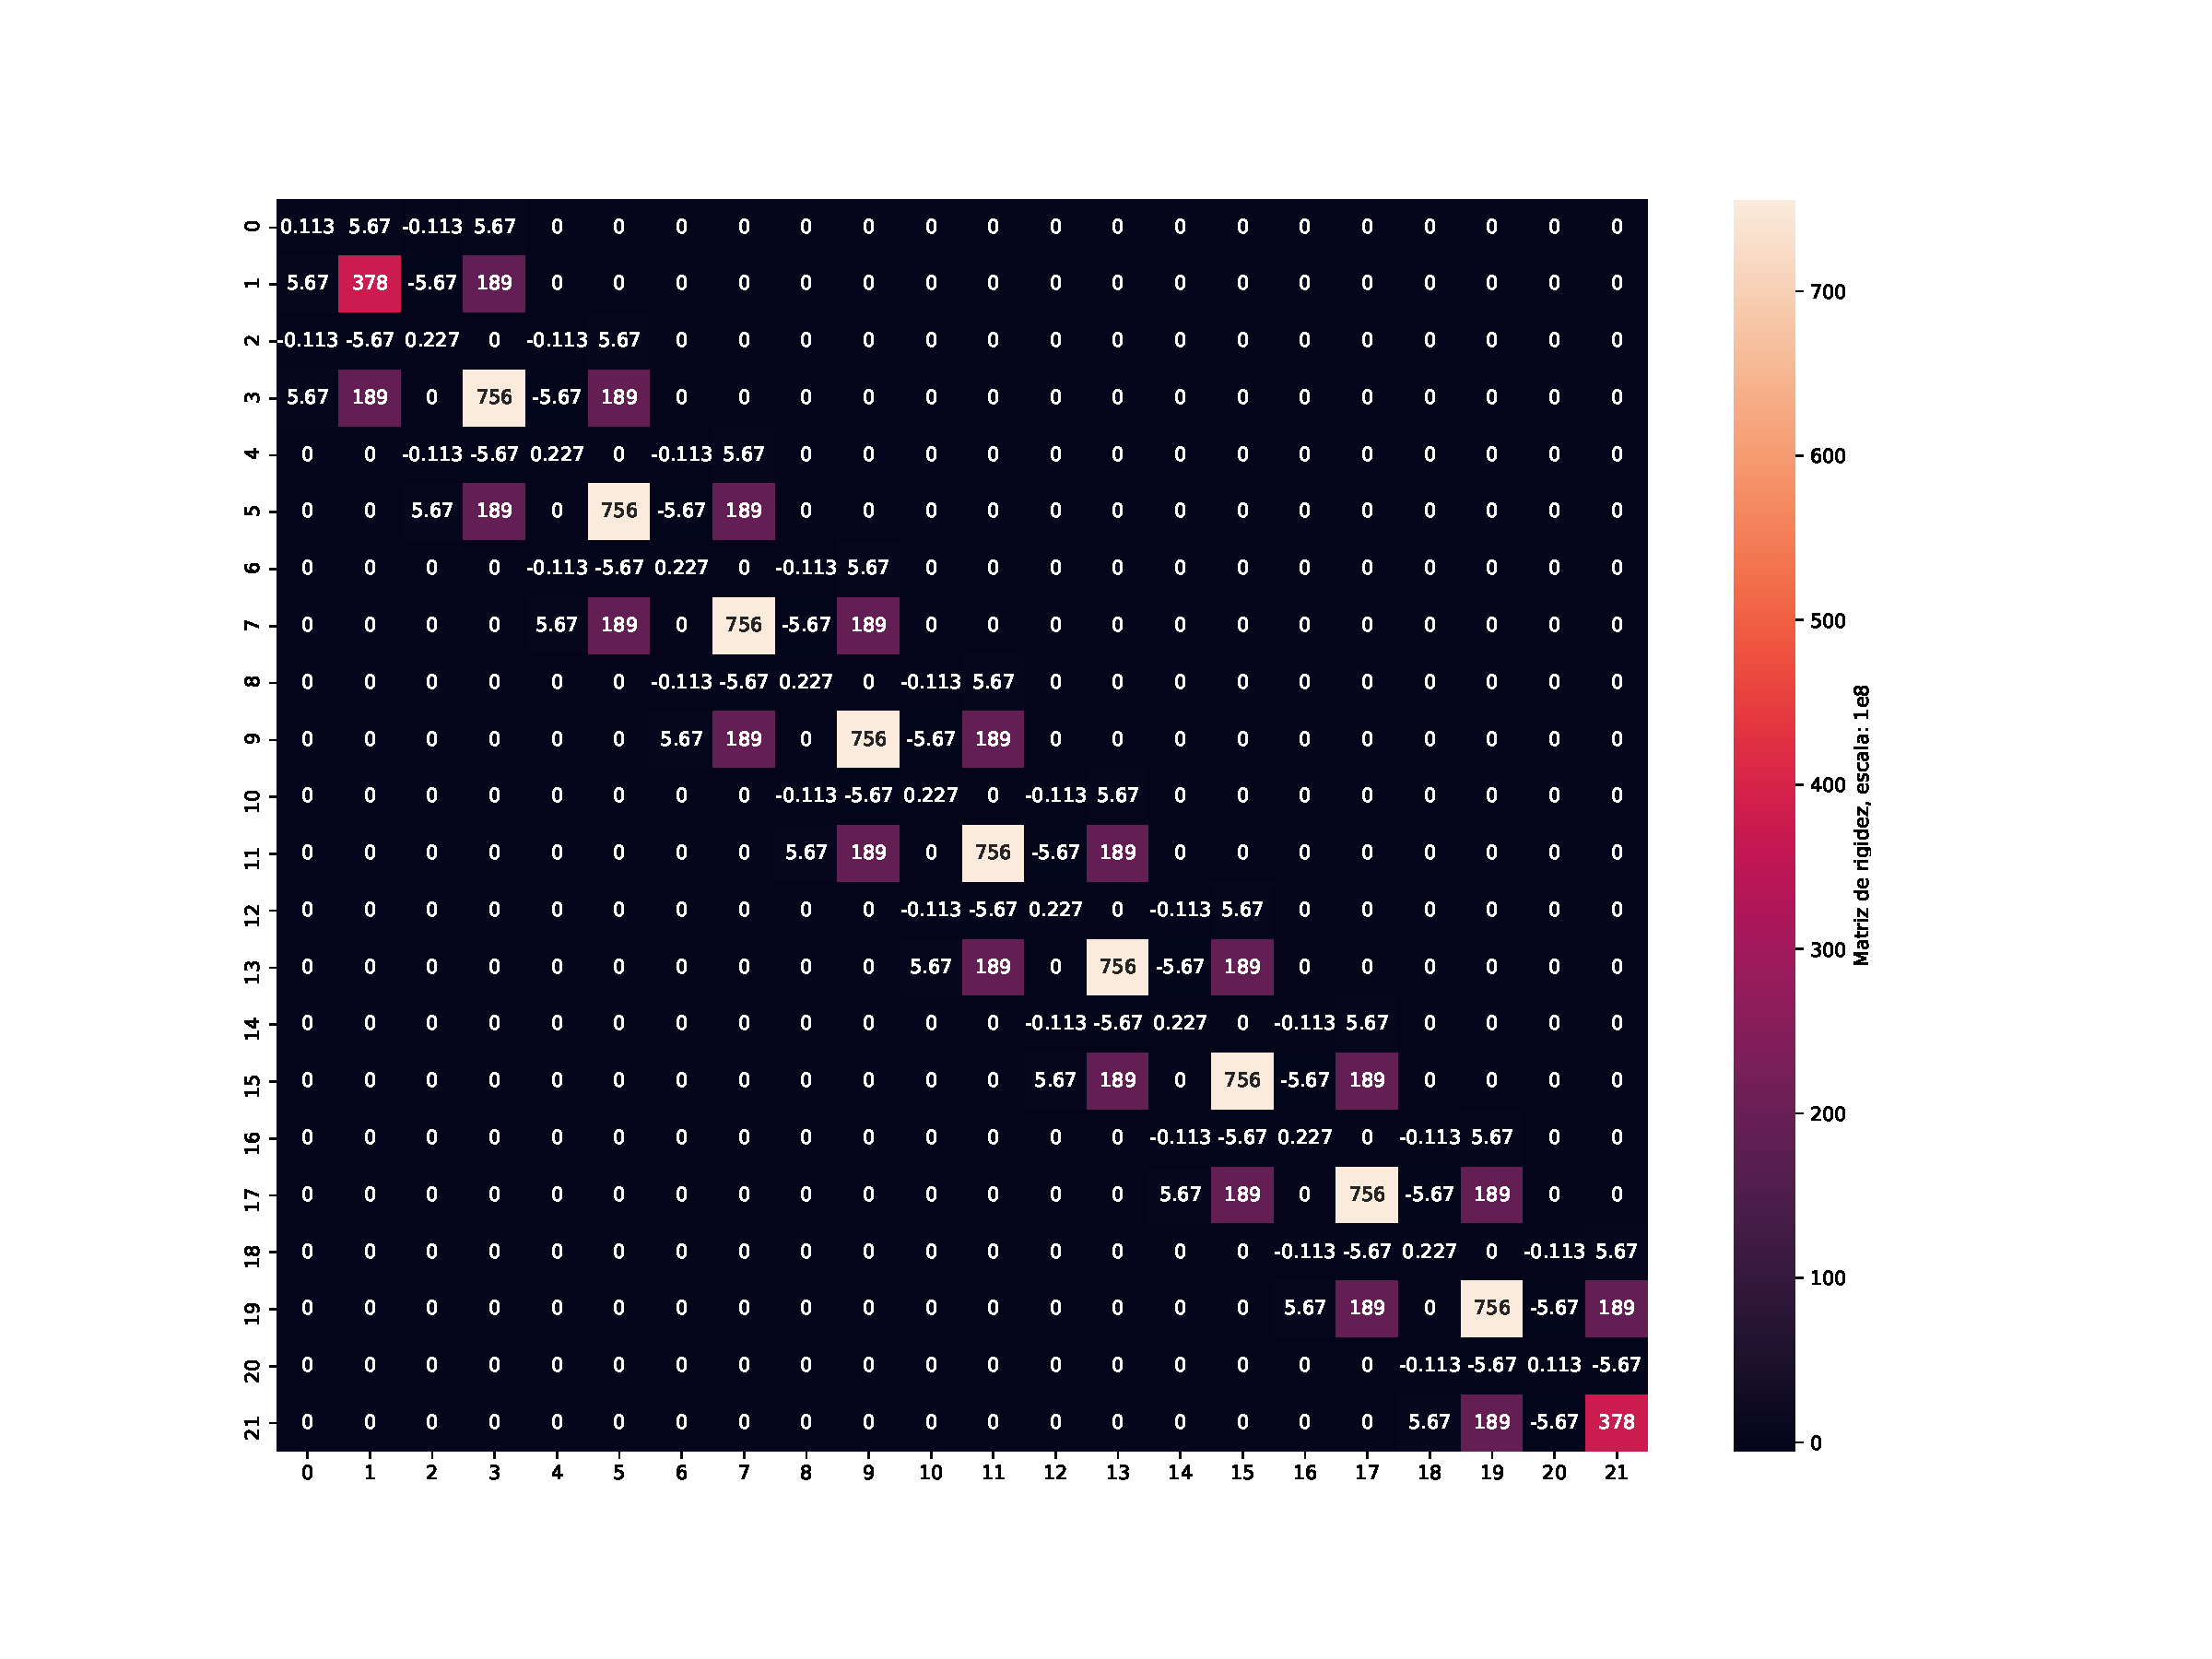
\includegraphics[scale=0.79]{stiffness.pdf}
    \caption{Matriz de rigidez}
\end{figure}
\begin{figure}[H]
    \centering
    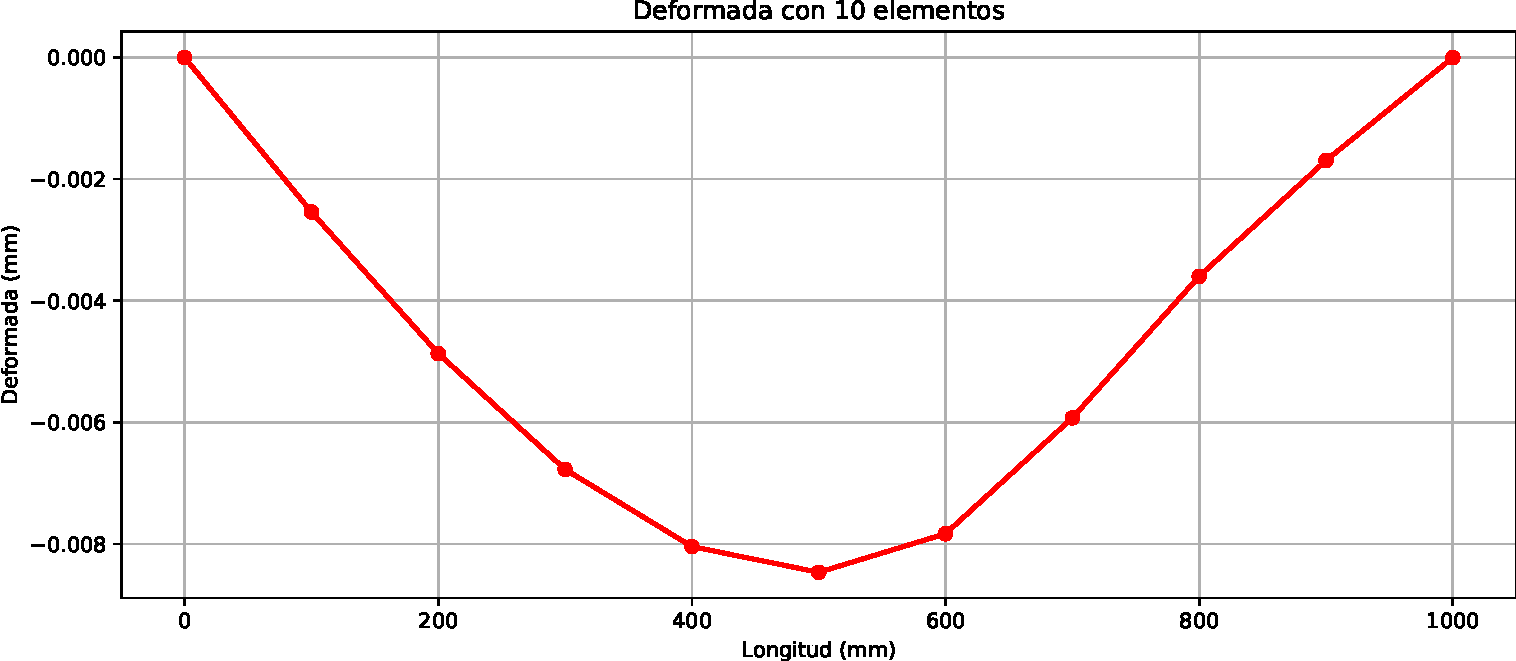
\includegraphics[scale=0.82]{displacements10.pdf}
    \caption{Deformada}
\end{figure}
\begin{figure}[H]
    \centering
    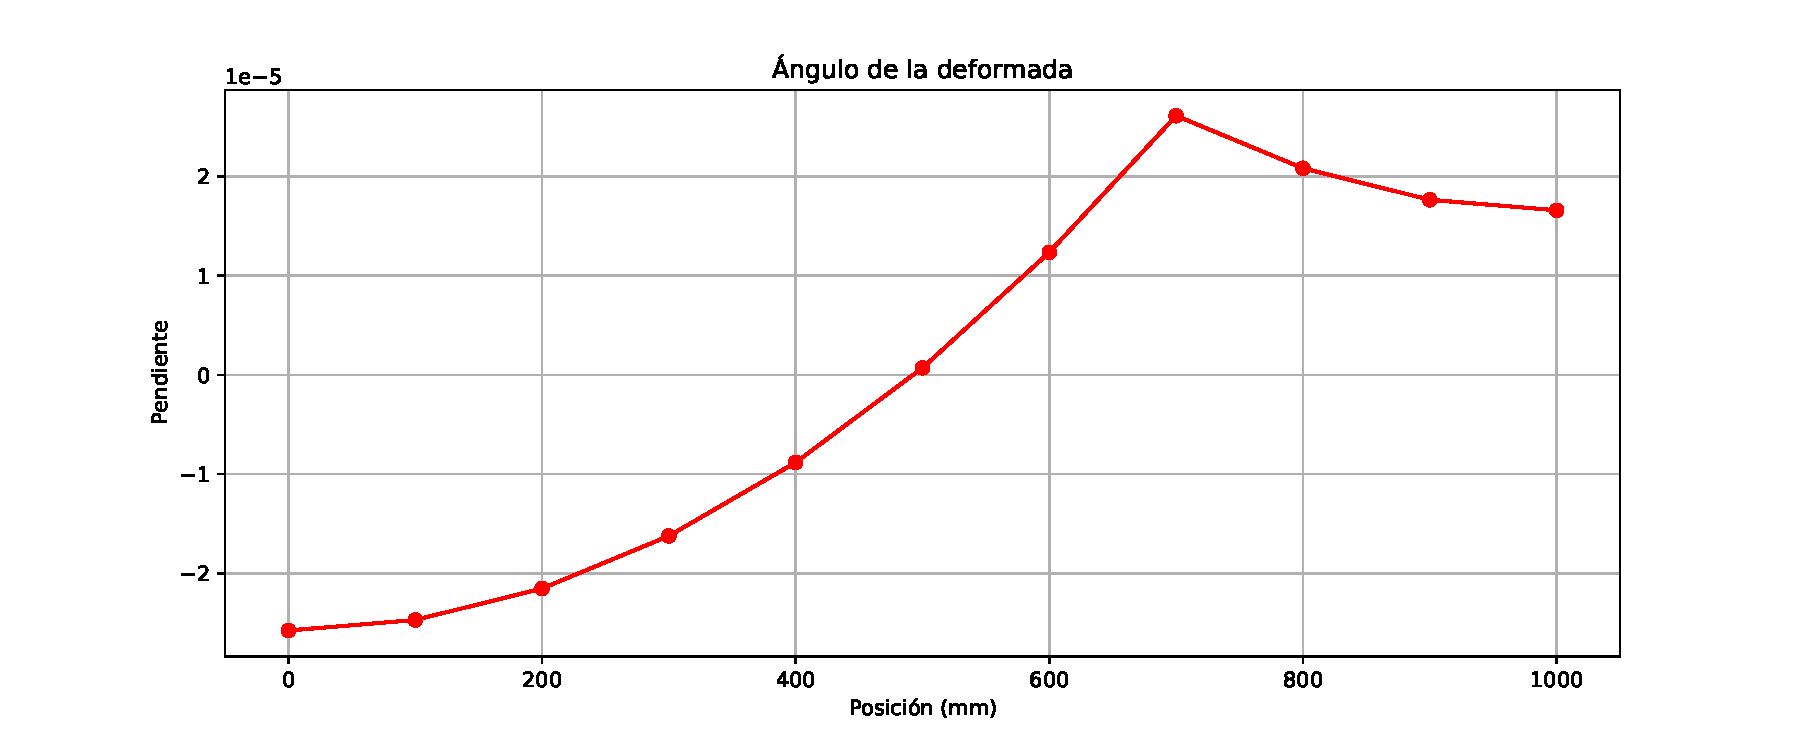
\includegraphics[scale=0.84]{angle10.pdf}
    \caption{Pendiente}
\end{figure}
Cada desplazamiento y fuerza corresponde a un nodo en una dirección ($y$ o $\theta$); por lo que al nodo $i$ le corresponde las reacciones $2i$ ($y$) y $2i+1$ ($\theta$).
Se organiza los datos del desplazamiento y fuerza en cada dirección en una tabla para cada nodo para tener una mejor compresión de los resultados:
\begin{table}[H]
    \centering
    \tcbox[left=0mm,right=0mm,top=0mm,bottom=0mm,boxsep=0mm,toptitle=0.8mm,bottomtitle=0.8mm,title=Resultados del análisis por elementos finitos]{
    \renewcommand{\arraystretch}{1.8}%
    \begin{tabular}{c|c|c||c|c}
        \hline
        Nodo & Desp. y (mm) & Desp. $\theta$ (rad) & Fuerza y (N) & Momento $\theta$ (N-mm)\\
        \hline
        0 & 0 & -25.8133 $\times 10^{-6}$ & 200 & 0 \\
        \hline
        1 & -2.54597 $\times 10^{-3}$ & -24.75248 $\times 10^{-6}$ & -2.18279 $\times 10^{-11}$ & 0 \\
        \hline
        2 & -4.87977 $\times 10^{-3}$ & -21.57001 $\times 10^{-6}$ & 7.09406 $\times 10^{-11}$ & -4.65661 $\times 10^{-10}$ \\
        \hline
        3 & -6.78925 $\times 10^{-3}$ & -16.26591 $\times 10^{-6}$ & -1.18234 $\times 10^{-11}$ & 6.98492 $\times 10^{-10}$ \\
        \hline
        4 & -8.06223 $\times 10^{-3}$ & -8.84017 $\times 10^{-6}$ & -1.63709 $\times 10^{-11}$ & 0 \\
        \hline
        5 & -8.48656 $\times 10^{-3}$ & 0.70721 $\times 10^{-6}$ & 0 & -3.63798 $\times 10^{-10}$ \\
        \hline
        6 & -7.85007 $\times 10^{-3}$ & 12.37624 $\times 10^{-6}$ & -4.18368 $\times 10^{-11}$ & 4.65661 $\times 10^{-10}$ \\
        \hline
        7 & -5.94059 $\times 10^{-3}$ & 26.1669 $\times 10^{-6}$ & 1.90994 $\times 10^{-11}$ & 200000\\
        \hline
        8 & -3.60679 $\times 10^{-3}$ & 20.8628 $\times 10^{-6}$ & 1.54614 $\times 10^{-11}$ & 0 \\
        \hline
        9 & -1.69731 $\times 10^{-3}$ & 17.68034 $\times 10^{-6}$ & -0.1819 $\times 10^{-11}$ & -1.16415 $\times 10^{-10}$ \\
        \hline
        10 & 0 & 16.61952 $\times 10^{-6}$ & -200 & 0
    \end{tabular}}
    \caption{Desplazamientos y reacciones en los nodos}
\end{table}
\begin{figure}[H]
    \centering
    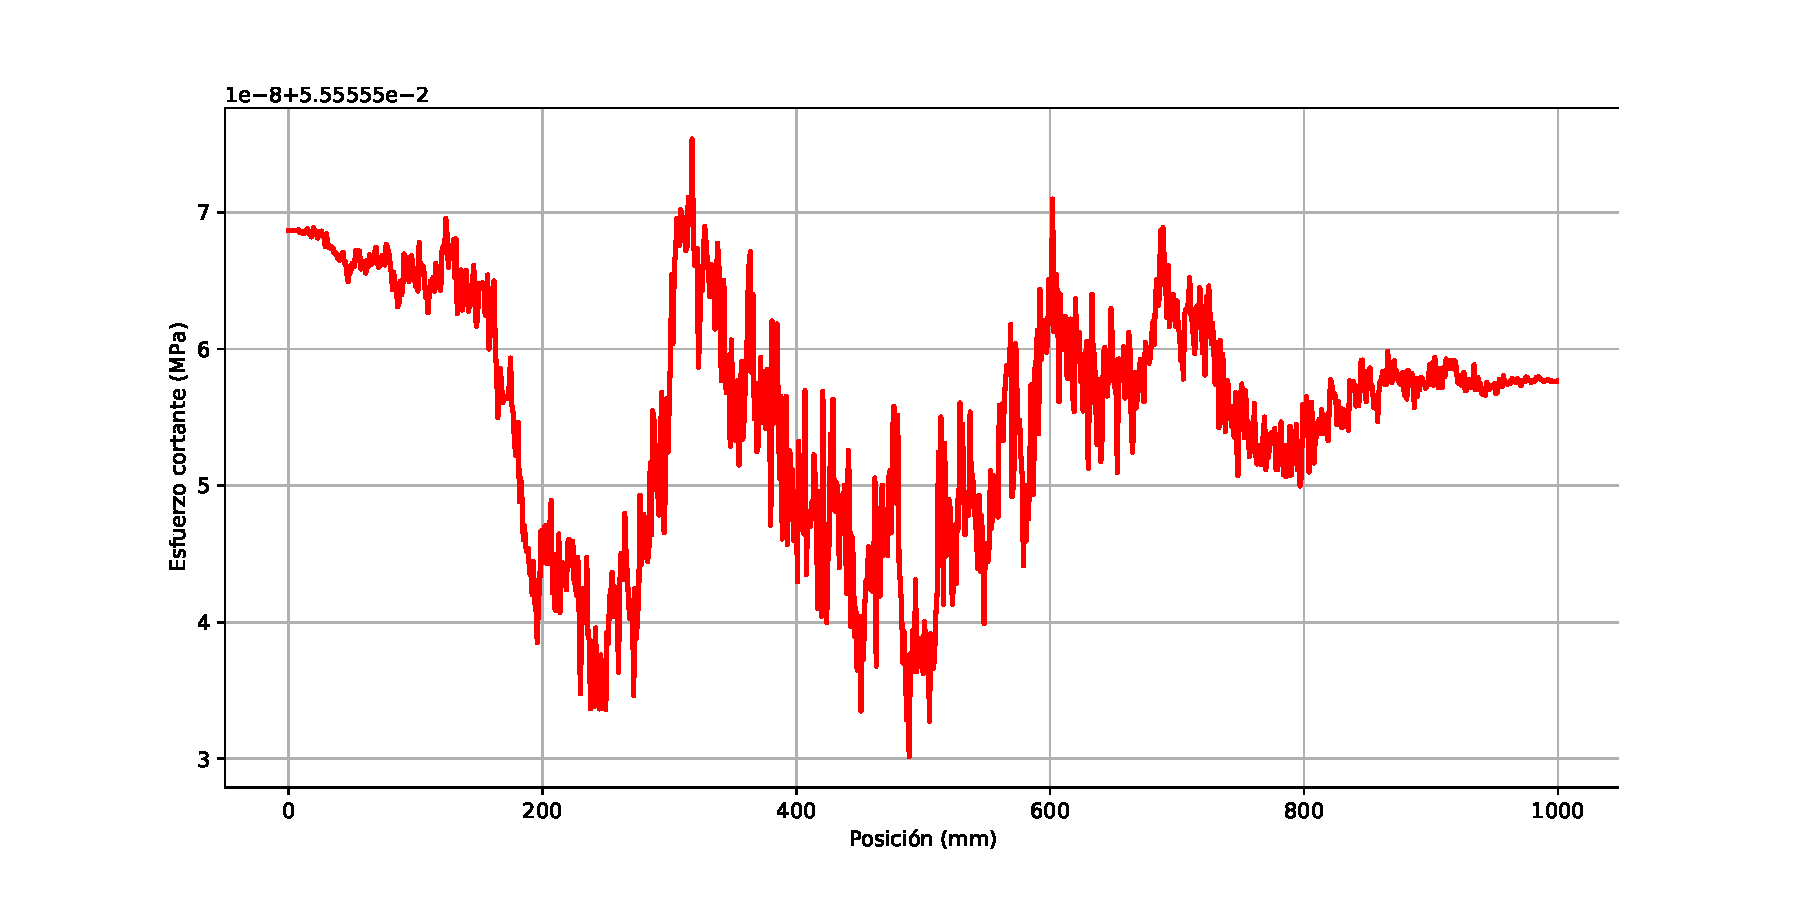
\includegraphics[scale=0.56]{stressC1.pdf}
    \caption{Error en el esfuerzo cortante}
\end{figure}
Debido a errores en la precisión del computador, se genera ruido en la solución, pero dichos errores son tan pequeños que son despreciables; eliminando el ruido de la gráfica, el esfuerzo cortante sería:
\begin{figure}[H]
    \centering
    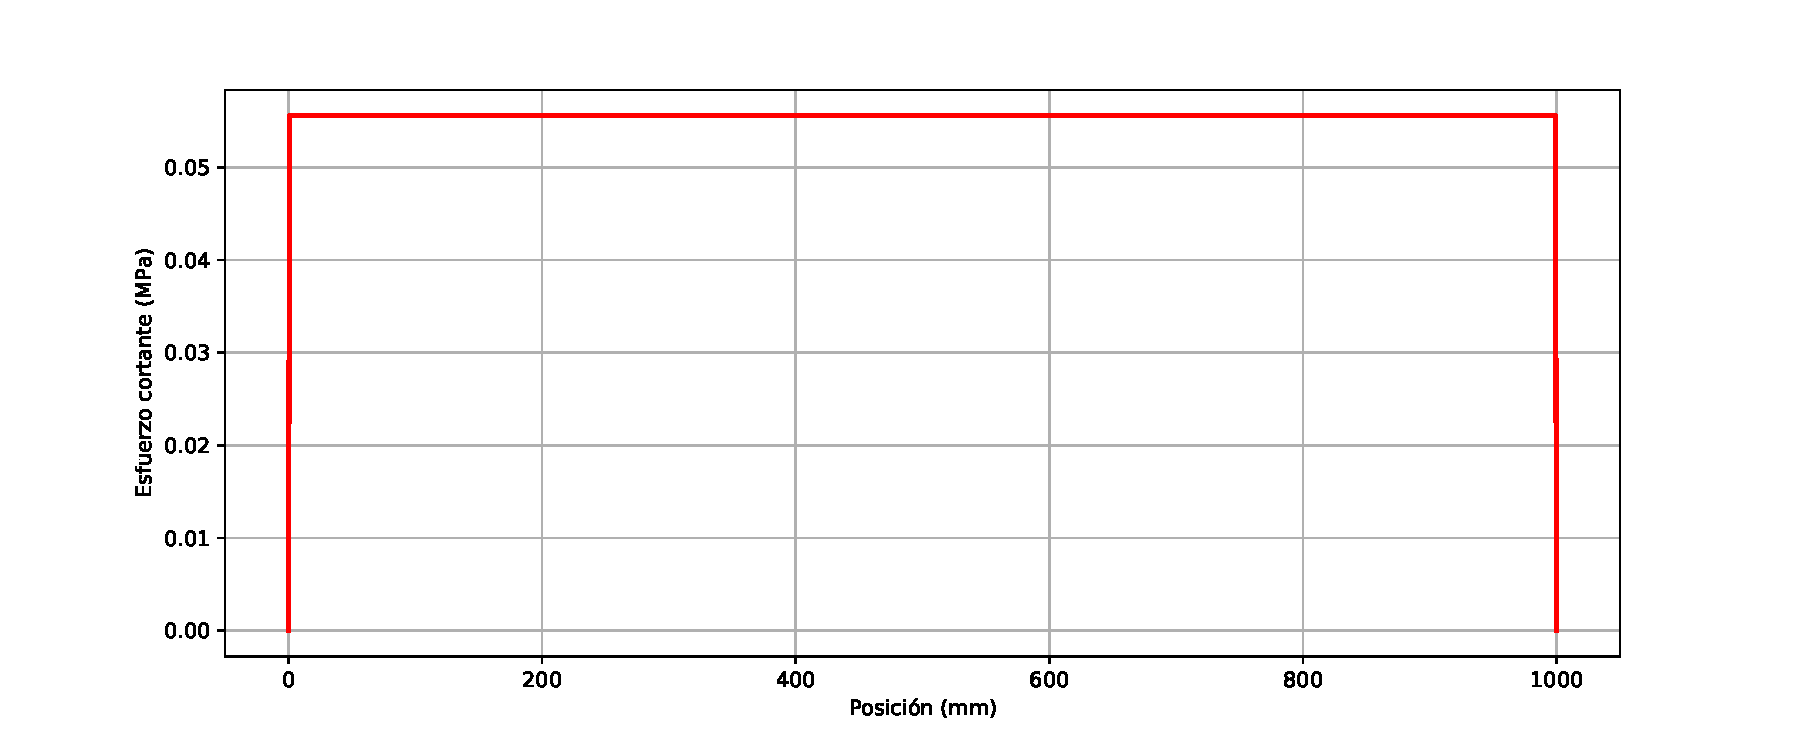
\includegraphics[scale=0.66]{stressC.pdf}
    \caption{Esfuerzo cortante}
\end{figure}
Mientras que el esfuerzo máximo por flexión sería:
\begin{figure}[H]
    \centering
    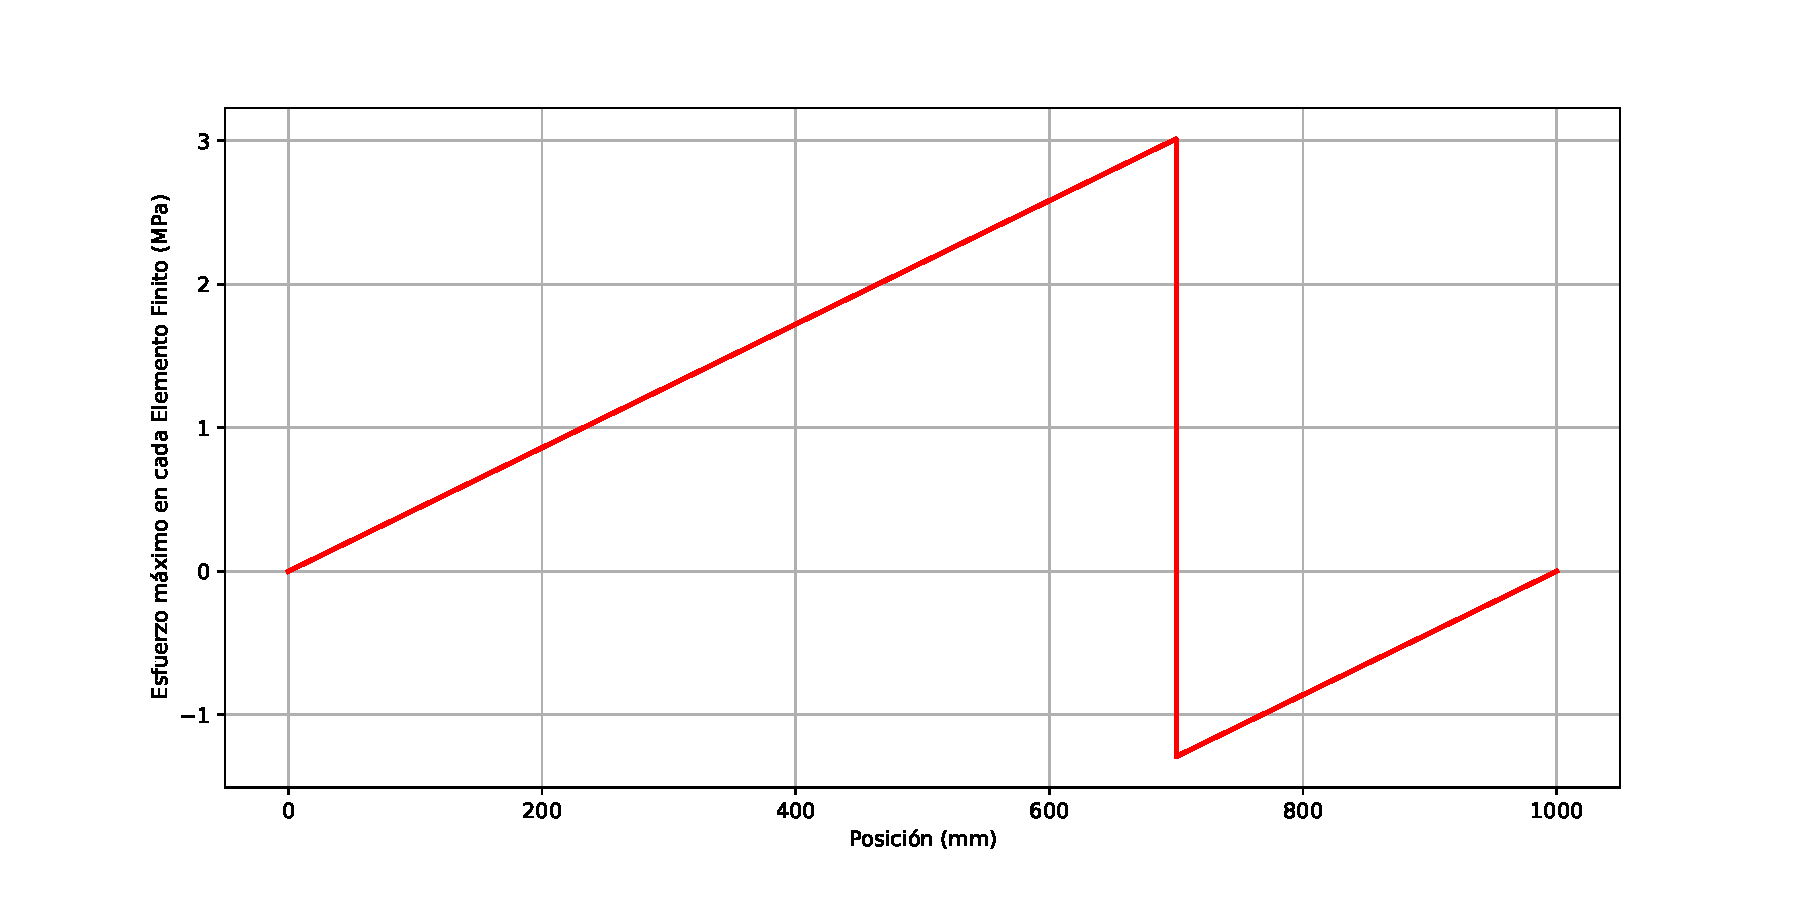
\includegraphics[scale=0.58]{stressT.pdf}
    \caption{Esfuerzo por flexión}
\end{figure}
Luego, los esfuerzos en cada elemento:
\begin{table}[H]
    \centering
    \tcbox[left=0mm,right=0mm,top=0mm,bottom=0mm,boxsep=0mm,toptitle=0.8mm,bottomtitle=0.8mm,title=Esfuerzos en los elementos]{
    \renewcommand{\arraystretch}{1}%
    \begin{tabular}{c||c|c||c||c|c}
        Elemento & Nodo 1 & Nodo 2 & Longitud & Esfuerzo por flexión (MPa) & Esfuerzo cortante (MPa)\\
        \hline
        0 & 0 & 1 & 100 mm& 0.4314 & 0.0555 \\
        \hline
        1 & 1 & 2 & 100 mm& 0.862801 & 0.0555 \\
        \hline
        2 & 2 & 3 & 100 mm& 1.294201 & 0.0555 \\
        \hline
        3 & 3 & 4 & 100 mm& 1.725601 & 0.0555 \\
        \hline
        4 & 4 & 5 & 100 mm& 2.157001 & 0.0555 \\
        \hline
        5 & 5 & 6 & 100 mm& 2.588402 & 0.0555 \\
        \hline
        6 & 6 & 7 & 100 mm& 3.019802 & 0.0555 \\
        \hline
        7 & 7 & 8 & 100 mm& -1.294201 & 0.0555 \\
        \hline
        8 & 8 & 9 & 100 mm& -0.862801 & 0.0555 \\
        \hline
        9 & 9 & 10 & 100 mm& -0.4314 & 0.0555
    \end{tabular}}
    \caption{Esfuerzos en la viga}
\end{table}
\section{Generalización para $\mathbf{n}$ elementos}
Al incrementar la cantidad de elementos se obtiene mayor información sobre la pendiente y la deformada en más secciones de la viga.
\begin{figure}[H]
    \centering
    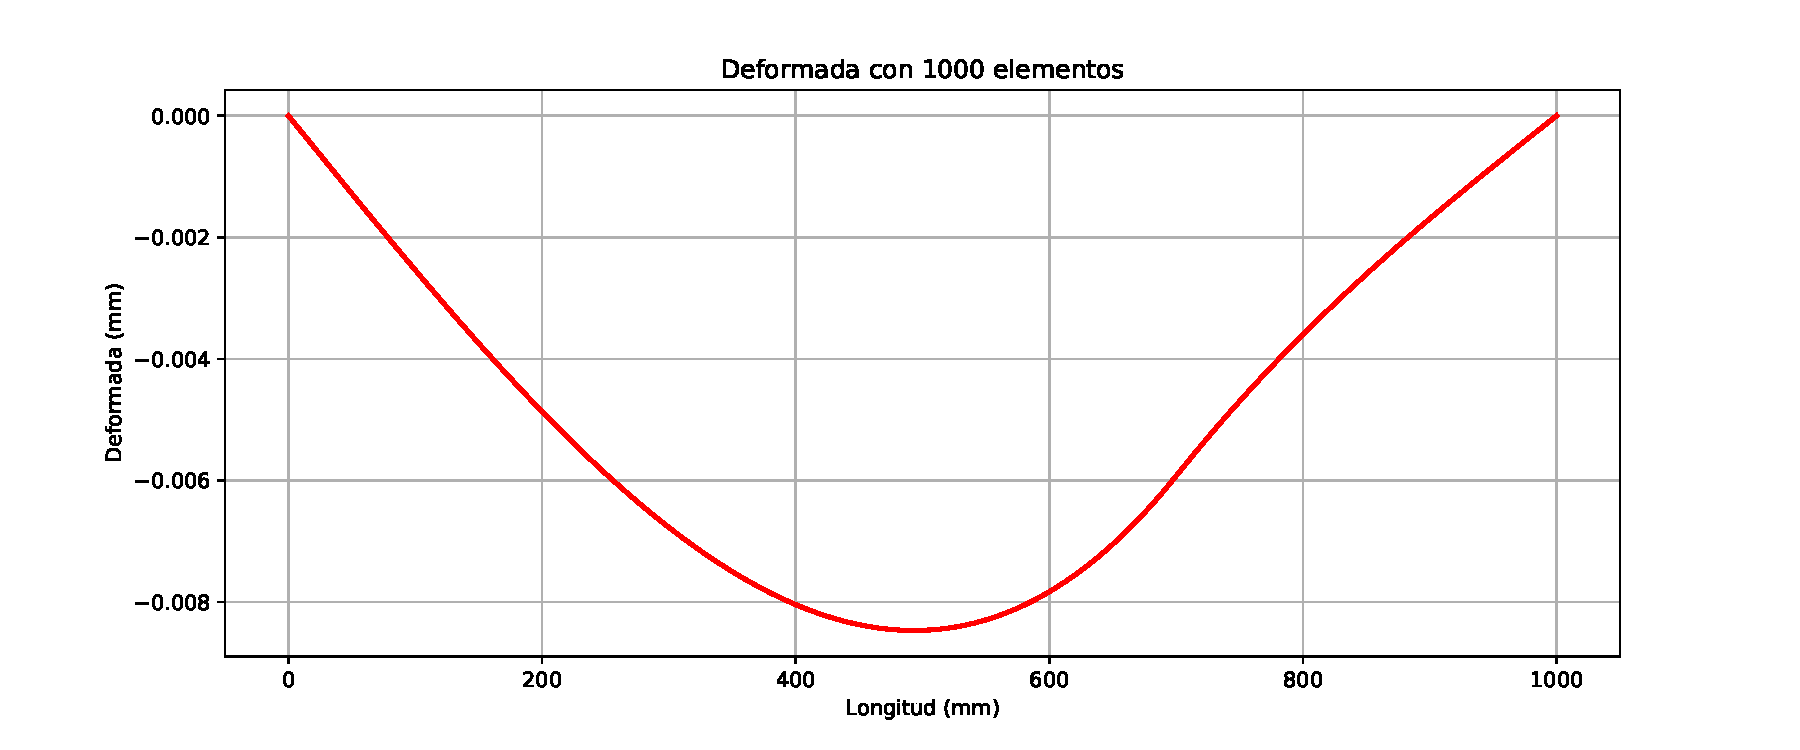
\includegraphics[scale=0.675]{displacements1000.pdf}
    \caption{Deformada para 1000 elementos}
\end{figure}
\begin{figure}[H]
    \centering
    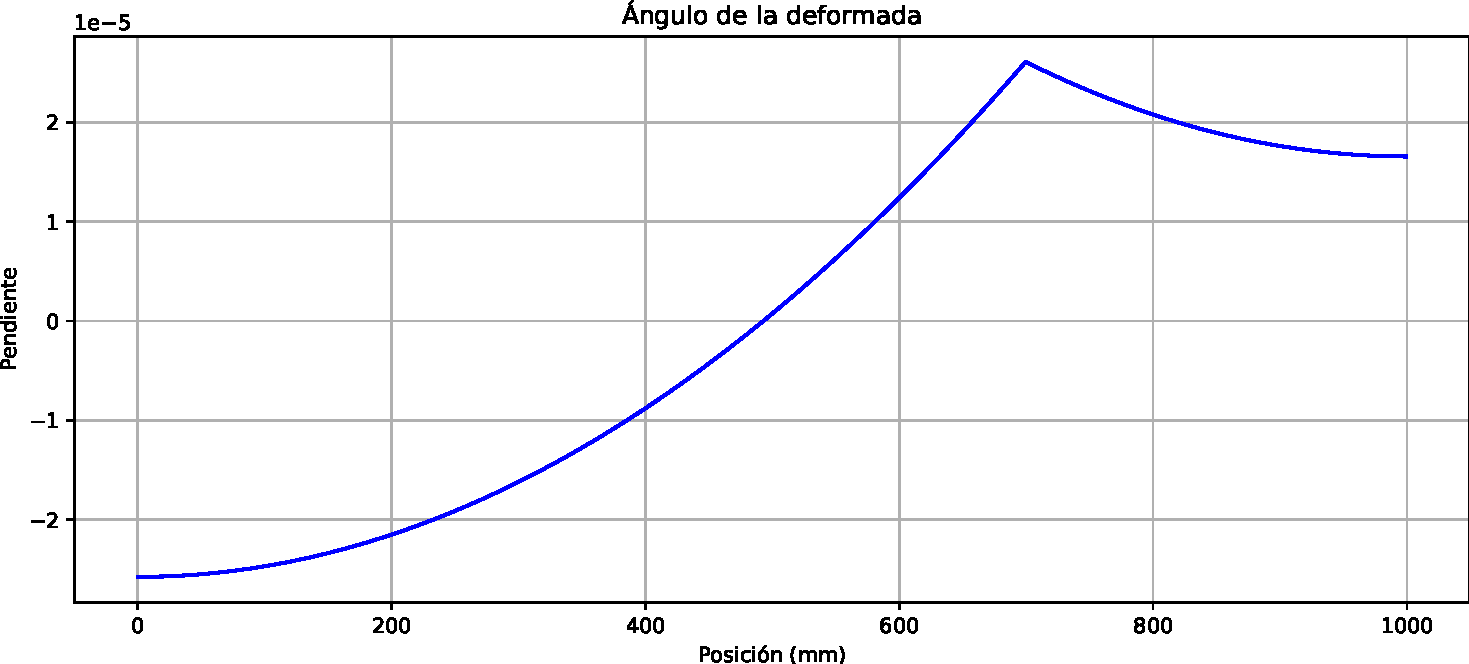
\includegraphics[scale=0.675]{angle1000.pdf}
    \caption{Pendiente para 1000 elementos}
\end{figure}
\section{Verificación de resultados en Autodesk Fusion 360}
Se modela la viga y sus apoyos en Fusion 360, para la verificación de resultados.
\begin{figure}[H]
    \centering
    \includegraphics[height=10.3cm,width=17.8cm]{deformation.PNG}
    \includegraphics[height=10.3cm,width=17.8cm]{maxdef.PNG}
    \caption{Deformación y flecha máxima de la viga a 493 mm}
\end{figure}
Los resultados son similares a los obtenidos con el código detallado en la sección 2. Tanto la flecha máxima como su posición en la viga coinciden con los resultados mostrados anteriormente.
\section{Verificación de resultados en SolidsPy}
Utilizando el software SolidsPy \cite{solidspy}; es posible modelar la viga con elementos cuadráticos de forma rápida y simple. Los resultados obtenidos se muestran a continuación:
\begin{figure}[H]
    \centering
    \includegraphics[height=10.2cm,width=17cm]{Horizontal_displacement.png}
    \includegraphics[height=10.2cm,width=17cm]{Vertical_displacement.png}
    \caption{Desplazamientos horizontales y verticales}
\end{figure}
El desplazamiento horizontal es pequeño y despreciable en comparación con la vertical; mientras que la vertical tiene un valor máximo de 0.008 mm cerca a 500 mm como se demostró en los resultados anteriores y a 700 mm ocurre una variación más atenuada de la pendiente, como se puede apreciar en la gráfica obtenida.
\section*{Convergencia del método de elementos finitos}
\begin{figure}[H]
    \centering
    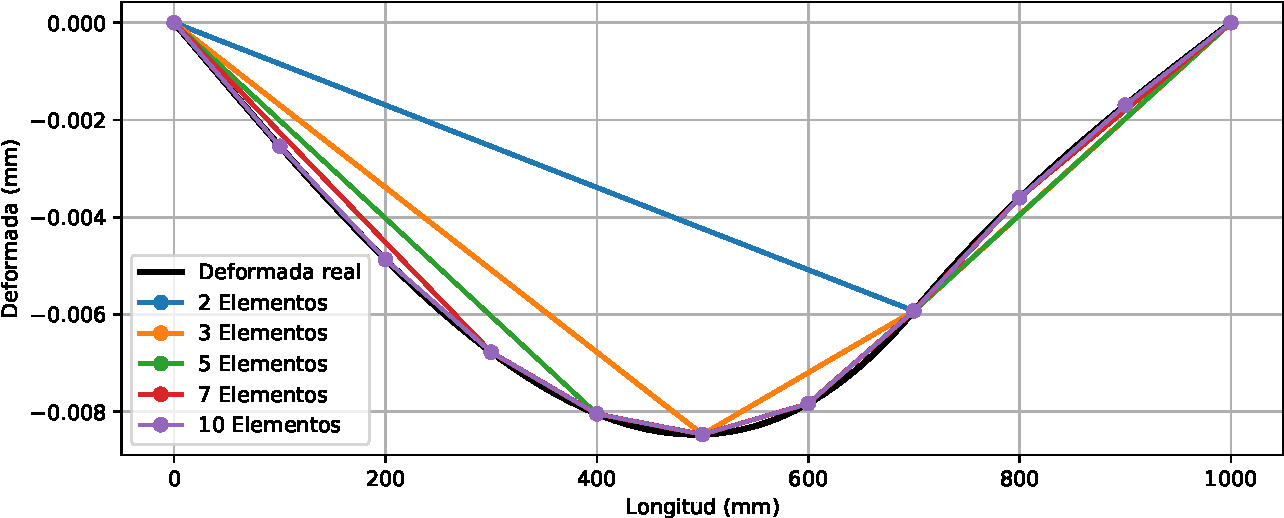
\includegraphics[scale=0.78]{comparision2.pdf}
    \caption{Convergencia de la deformada al aumentar los elementos}
\end{figure}
\section*{Optimización del mallado}
Se observa que la flecha máxima se encuentra entre 400 y 500 mm. Para obtener una mayor precisión de la ubicación de la flecha puede aumentarse el mallado, pero esto crearía demasiados elementos, entonces solo se mejora el mallado entre una región más pequeña, mientras que en las otras secciones de la viga el mallado sigue como antes.
\begin{figure}[H]
    \centering
    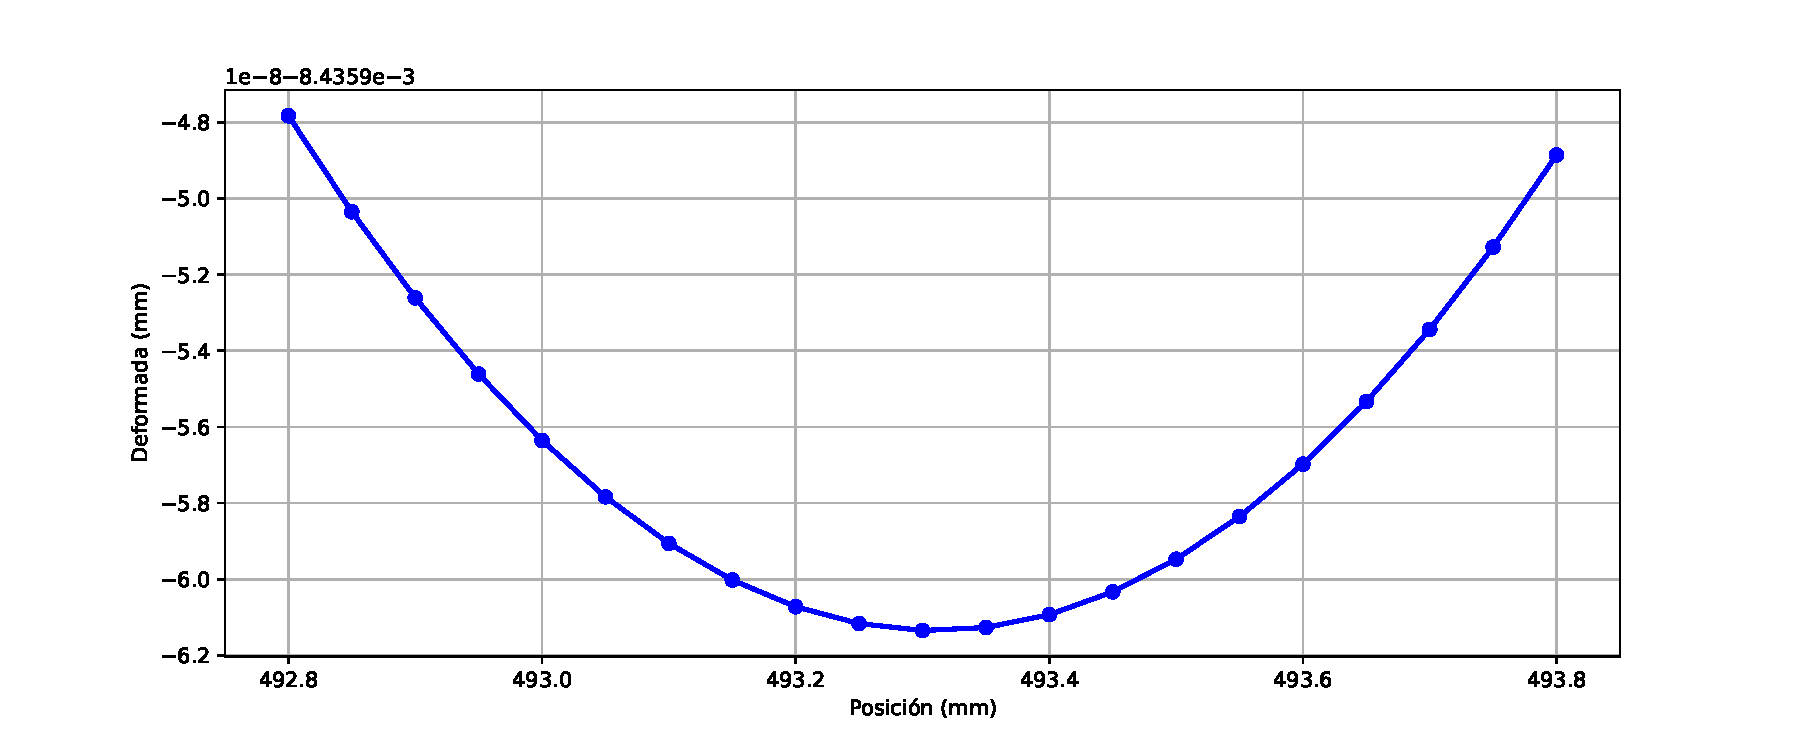
\includegraphics[scale=0.69]{refinament1.pdf}
    \caption{Refinamiento del mallado entre 490 y 500 mm}
\end{figure}
La flecha máxima está alrededor de 493.3 y tiene un valor de 0.0084889288 mm, similar al resultado obtenido de forma analítica. Con un error relativo igual a 0.000048125\%.
\section*{Análisis por diferencias finitas}
La viga también puede desarrollarse al seguir un procedimiento similar a como se hizo para el curso MC325, utilizando el código de \cite{finite_difference} donde se puede usar el método de diferencias finitas para obtener una solución aproximada de la ecuación diferencial de la deformada. 
\begin{figure}[H]
    \centering
    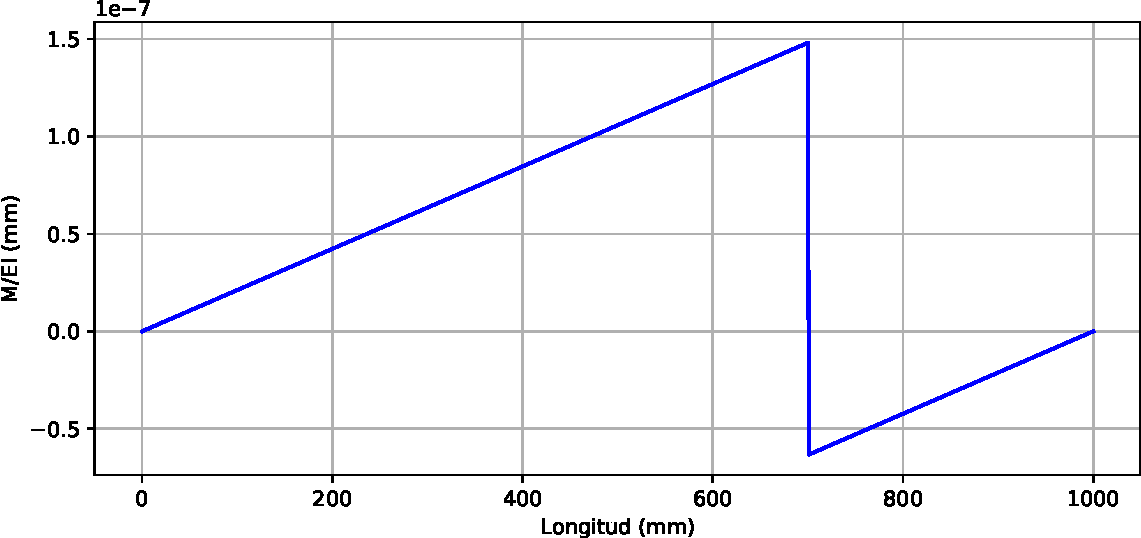
\includegraphics[scale=0.78]{mei.pdf}
    \caption{M/EI}
\end{figure}
\begin{figure}[H]
    \centering
    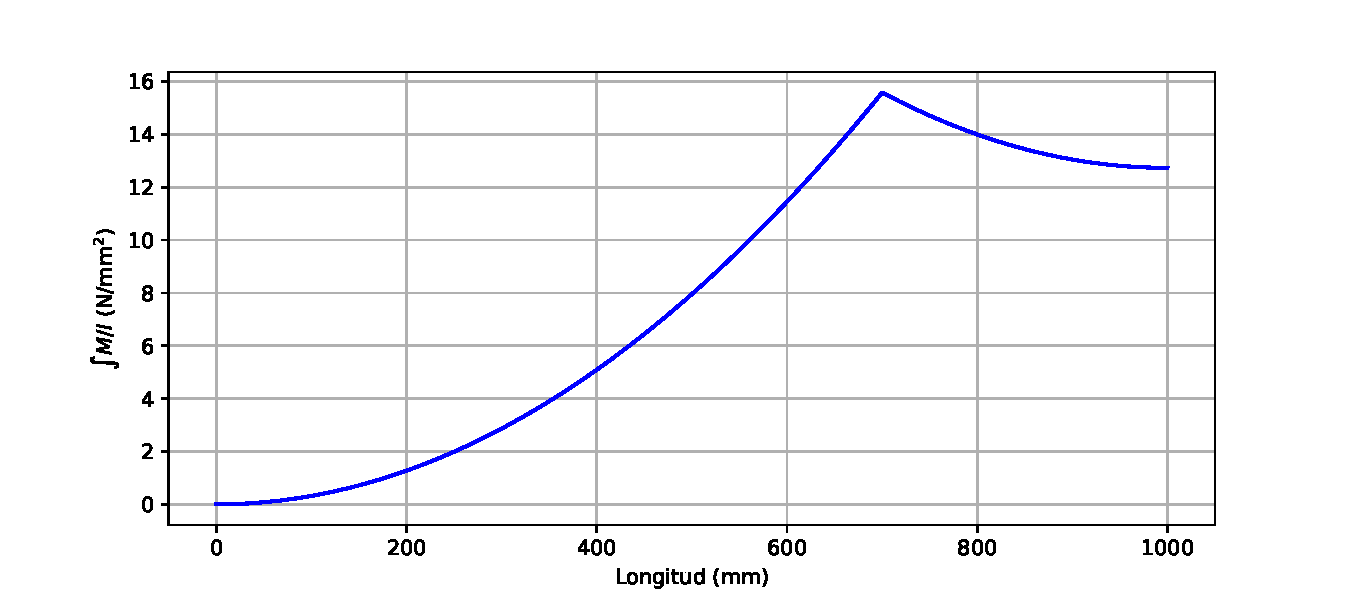
\includegraphics[scale=0.78]{mi.pdf}
    \caption{$\int M/I$}
\end{figure}
\begin{figure}[H]
    \centering
    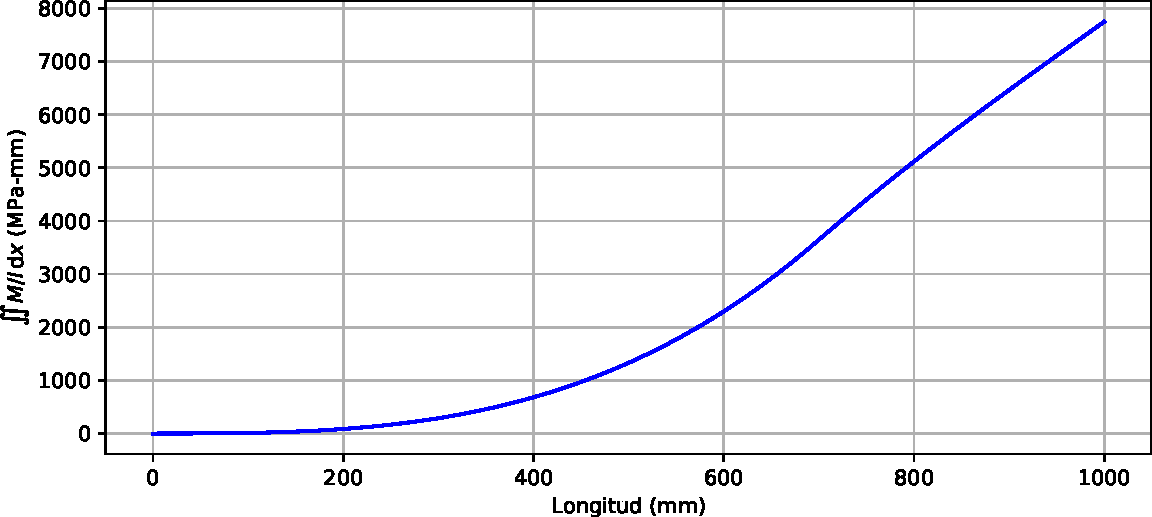
\includegraphics[scale=0.78]{mii.pdf}
    \caption{$\iint M/I$}
\end{figure}
Dado que la integral $\iint M/I$ contiene constantes, es necesario hallarlas y añadirlas a la gráfica final para obtener la deformada:
\begin{figure}[H]
    \centering
    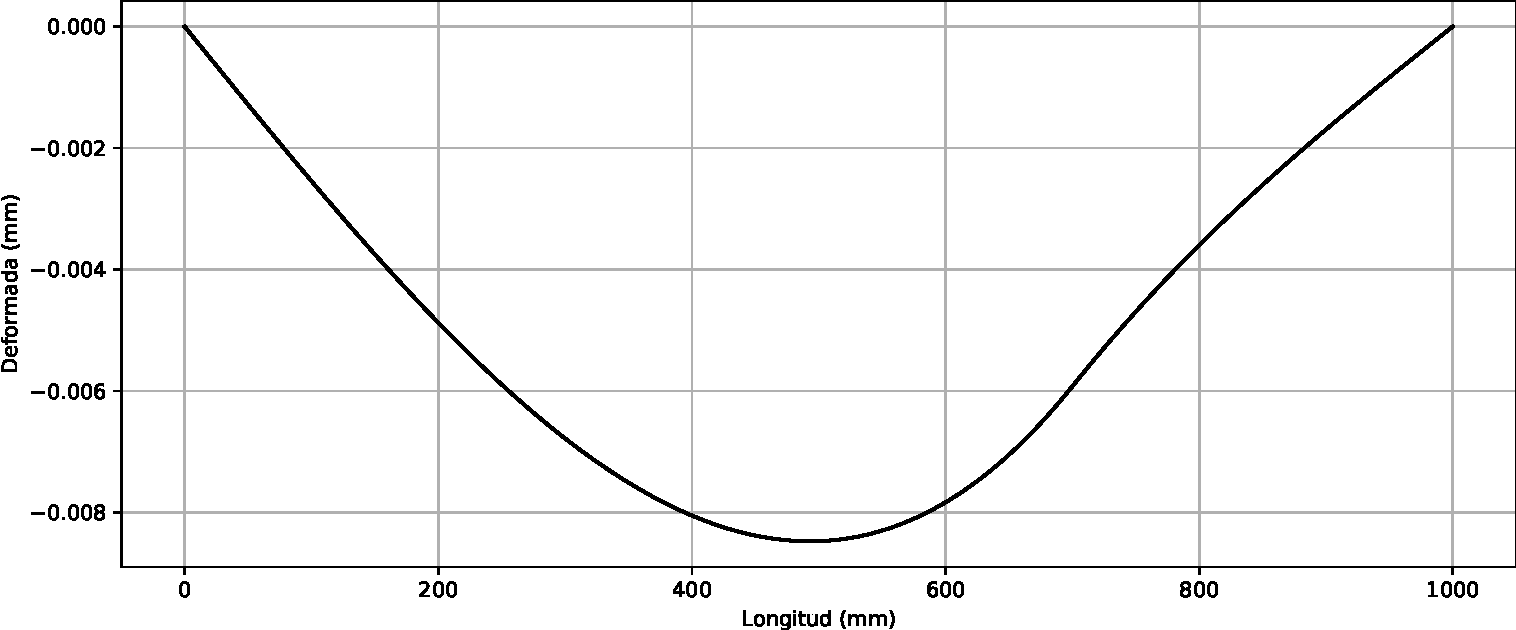
\includegraphics[scale=0.8]{deformada1000.pdf}
    \caption{Deformada obtenida por diferencias finitas}
\end{figure}
\section*{Comparación entre diferencias finitas y elementos finitos}
El método de diferencias finitas es la implementación de un clásico algoritmo DP, en el que se reutiliza estados anteriores para formar nuevos y así completar la solución completa. En este caso el algoritmo utiliza el estado anterior para así reconstruir la solución; es decir, es el método de Euler para la solución de una ecuación diferencial. Este método tiene una complejidad de tiempo $O(n)$ y la memoria puede optimizarse a $O(1)$, pero su convergencia a la solución es $O(n)$. Existen métodos más eficientes que utilizan aproximaciones más exactas para obtener una convergencia de $O(n^{2})$. Mientras que el método de elementos finitos aproxima la región obteniendo una convergencia igual al grado de la solución analítica, es decir $O(n^{3}/6)$ pero con un uso de memoria $O(n^{2})$ y un tiempo de ejecución de $O(n^{3})$, con las optimizaciones que se realizan en el código fue posible reducir el tiempo de ejecución a $O(n^{2}\log(n))$. Existen optimizaciones más poderosas para elementos finitos que reducen el uso de memoria excesivo usando una estructura de datos \cite{sparse_code} que elimina regiones de la matriz que son iguales a 0, de esa forma es posible usar más elementos y segmentar la solución. Como tal, el método de elementos finitos presenta un mejor desarrollo para resolver problemas donde la convergencia obtenida puede ser muy alta, como es el caso de la viga. Esto puede observarse en la siguiente gráfica:
\begin{figure}[H]
    \centering
    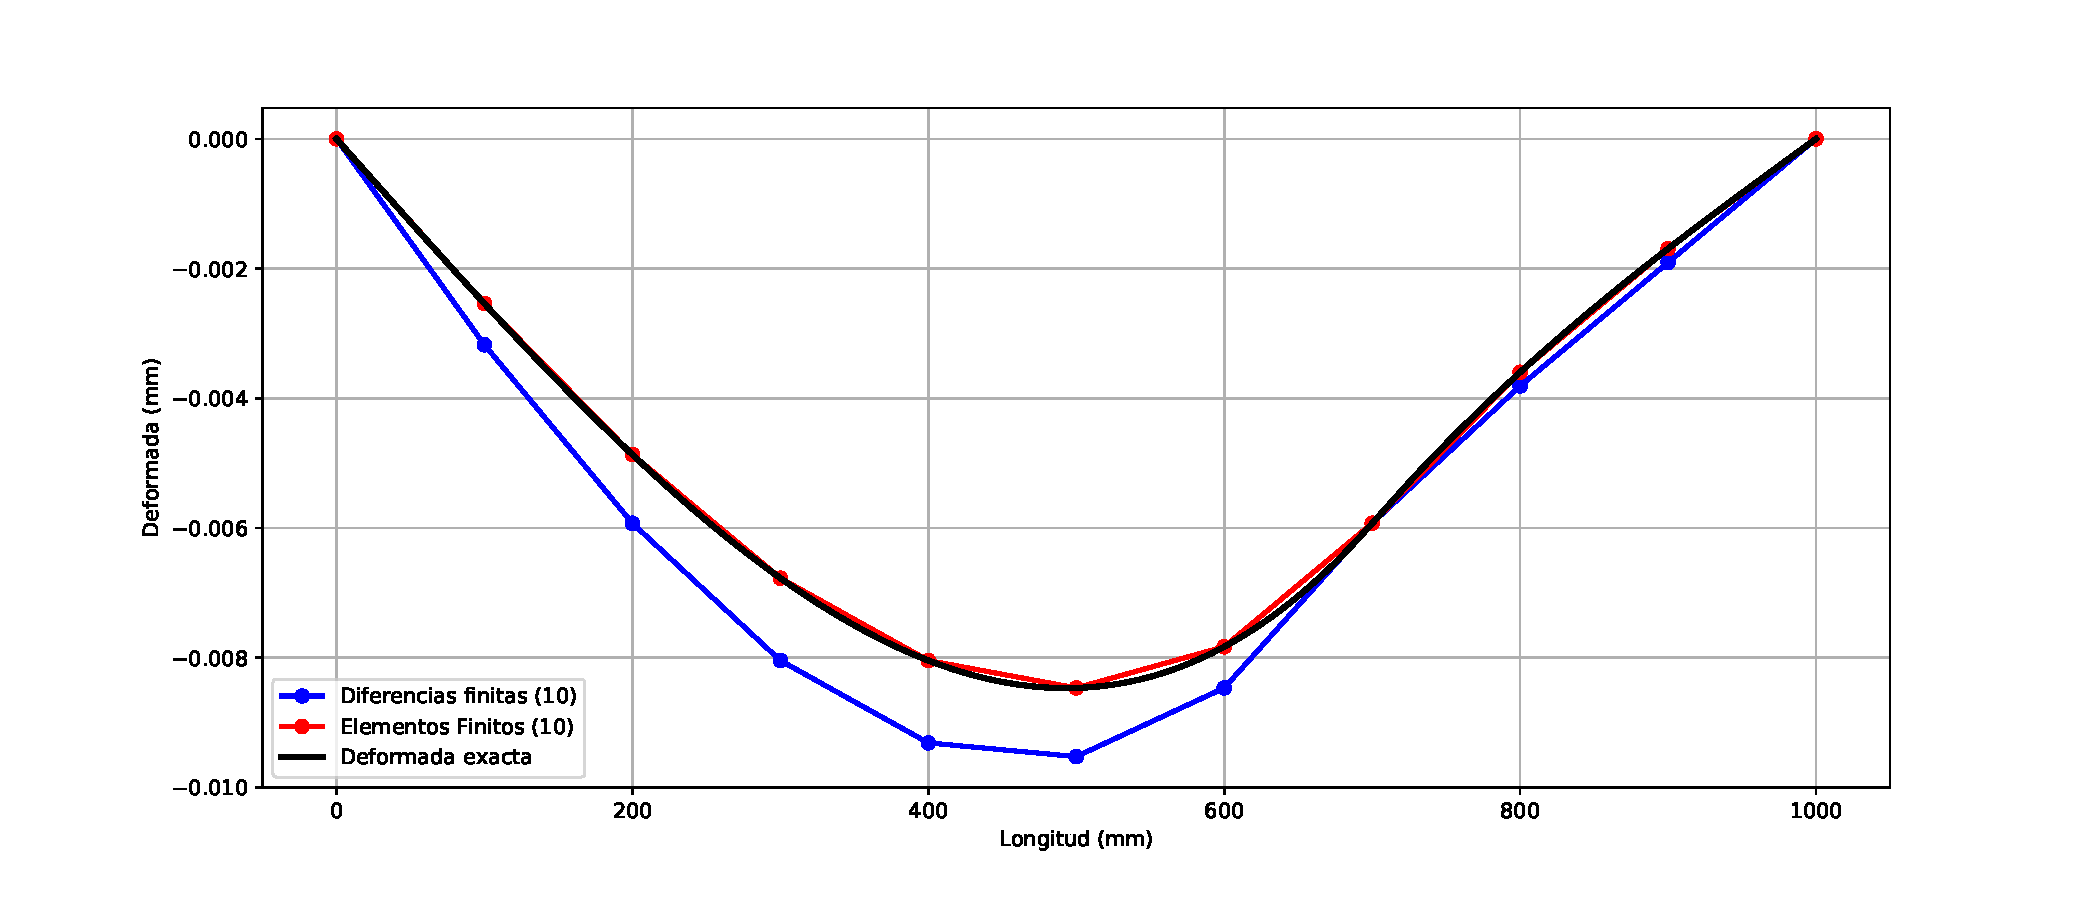
\includegraphics[scale=0.57]{comparision.pdf}
    \caption{Comparación entre el método de diferencias finitas y elementos finitos}
\end{figure}
El método de elementos finitos con solo 10 elementos está más cerca a la deformada que el método de diferencias finitas con la misma cantidad; se observa que para obtener una convergencia similar sería necesario usar alrededor de 1000 elementos en diferencias finitas, haciendo que el método de elementos finitos sea mucho más eficiente.
\begin{figure}[H]
    \centering
    \includegraphics[scale=0.76]{wtf.pdf}
    \caption{Comparación entre el método de diferencias finitas y elementos finitos}
\end{figure}

\begin{table}[H]
    \centering
    \tcbox[left=0mm,right=0mm,top=0mm,bottom=0mm,boxsep=0mm,toptitle=0.8mm,bottomtitle=0.8mm,title=Elementos finitos y Diferencias finitas]{
    \renewcommand{\arraystretch}{1}%
    \begin{tabular}{c||c|c}
        \textbf{Características} & \textbf{Diferencias finitas} & \textbf{Elementos finitos}\\
        \hline
        \textbf{Tiempo de ejecución} & $O(n)$ & $O(n^{2}\log(n))$ \\
        \hline
        \textbf{Uso de memoria} & $O(1)$ & $O(n^{2})$ \\
        \hline
        \textbf{Convergencia} & $O(n)$ & $O(n^{3})$
    \end{tabular}}
    \caption{Comparación entre Elementos finitos y Diferencias finitas}
\end{table}
Además, existen métodos numéricos \cite{fast_algorithms} que pueden obtener una convergencia similar a elementos finitos con un tiempo de ejecución similar, dichos métodos son llamados multilinear-step y son usados como una generalización al método de Euler. 

\section*{Conclusiones}
\begin{enumerate}
    \item Se logró verificar que el método de elementos finitos es capaz de dar resultados precisos aún con pocos elementos. Teniendo un error de menos del 0.05\% con solo 10 elementos.
    \item Tanto SolidsPy como Fusion 360, otorgan resultados similares aún cuando su mallado fue cuadrático y tetraédrico respectivamente. Sin embargo, se espera que el elemento viga tenga una mayor convergencia y rapidez en los cálculos.
    \item Debido a que la longitud de la viga es relativamente grande, para obtener mayor precisión de la posición de la flecha máxima en la viga es necesario hacer un refinamiento de mallado, previa obtención de los resultados con menos elementos.
    \item Logra demostrarse de forma efectiva que el método de elementos finitos tiene una convergencia superior al método de Euler de primer orden.
    \item Se observa que, aunque el método de elementos finitos tiene una complejidad en ejecución muy alta, es posible optimizar el método con estructuras de datos más sofisticadas \cite{sparse_code} reduciendo el tiempo de ejecución a la quinta parte que en una implementación común.
    \item El tiempo de ejecución en un lenguaje de bajo nivel como C++, es alta debido a que el método del gradiente conjugado utilizó varios pasos hasta converger. Sin embargo, sigue siendo aún más rápido que Python o MATLAB.
\end{enumerate}


\bibliographystyle{IEEEtran}
\bibliography{IEEEabrv,sample}
\end{document}
